\section{Introduction}
\label{section:intro}
Although enormous amounts of data exist in ``well-behaved'' formats such
as relational tables and XML, massive amounts also exist in
non-standard or \textit{ad hoc} data formats. \tblref{figure:data-sources}
gives some sense of the range and pervasiveness of such data.
Ad hoc data comes in many forms: ASCII, binary, EBCDIC, and mixed
formats.  It can be fixed-width, fixed-column, variable-width, or even
tree-structured.  It is often quite large, including some data sources
that generate over a gigabit per second~\cite{gigascope}. It frequently
comes with incomplete and/or out-of-date documentation, and there are
almost always errors in the data.  Sometimes these errors are the most
interesting aspect of the data, \eg{}, in log files where
errors indicate that something is going wrong in the associated
system.

\begin{table}
\begin{center}
\begin{tabular}{l|l}
\hline
\textbf{Name} : Use   &  Representation               \\ \hline
\textbf{Web server logs (CLF)}:  &  Fixed-column ASCII records \\ 
Measure web workloads &                             \\ \hline
\textbf{AT\&T provisioning data}: & Variable-width ASCII records  \\ 
Monitor service activation &                              \\ \hline
\textbf{Call detail}: Fraud detection  &  Fixed-width binary records \\  \hline 
\textbf{AT\&T billing data}: & Various Cobol data formats  \\ 
Monitor billing process   &                             \\ \hline
\textbf{Netflow}:            & Data-dependent number of     \\ 
Monitor network performance  & fixed-width binary records  \\ \hline
\textbf{Newick}:   Immune  & Fixed-width ASCII records \\ 
system response simulation & in tree-shaped hierarchy\\ \hline                                
\textbf{Gene Ontology}:    & Variable-width ASCII records \\
Gene-gene correlations     & in DAG-shaped hierarchy \\ \hline
\textbf{OPRA}:              & Mixed binary \& ASCII records \\
Options-market transactions & with data-dependent unions \\ \hline
%IP backbone data:  & ASCII   \\
%Monitor network performance  &        \\ \hline
%HL7:             & Variable-width ASCII records \\
%Medical lab results     &  \\ \hline
% \textbf{CPT codes}: Medical diagnoses & Floating point numbers \\ \hline
% \textbf{SnowMed}: Medical clinic notes & Keyword tags  \\ 
\end{tabular}
\caption{Selected ad hoc data sources.}
\label{figure:data-sources}
\end{center}
\end{table}

The lack of standard tools for processing ad hoc data forces
analysts to roll their own tools, leading to scenarios such as the
following.  An analyst receives a new ad hoc data source containing
potentially interesting information and a list of pressing questions
about that data.  Could she please provide the answers to the
questions as quickly as possible, preferably last week?  The
accompanying documentation is outdated and incomplete, so she first has to experiment with the data to discover
its structure.   Eventually, she understands the data well enough to hand-code a
parser, usually in \C{} or \perl{}.  Pressed for time, she interleaves
code to compute the answers to the supplied questions with the parser.
As soon as the answers are computed, she gets a new data source and a
new set of questions to answer.

Through her heroic efforts, the data analyst answered the necessary
questions, but the approach is deficient in many respects.  The
analyst's hard-won understanding of the data is embedded in a
hand-written parser, where it is difficult for others to benefit from
her understanding.  The parser is likely to be brittle with respect to
changes in the input sources.  Consider, for example, how tricky it is
to figure out which \$3's should be \$4's in a \perl{} parser when a
new column appears in the data.  Errors in the data also pose a
significant challenge in hand-coded parsers.  If the data analyst
thoroughly checks for errors, then the error checking code dominates
the parser, making it even more difficult to understand the semantics
of the data format.  If she is not thorough, then erroneous data can
escape undetected, potentially (silently!)  corrupting down-stream
data processing.  Finally, in
answering the specified questions, the analyst had to code \textit{how
to compute} the questions rather than being able to express the
queries in a declarative fashion.  Many of these pitfalls
can be avoided with careful design and sufficient time, but such
luxuries are not available to the analyst.  However, with the
appropriate tool support, many aspects of this process can be greatly
simplified.

The \pads{} system~\cite{fisher+:pldi05} allows analysts to describe
ad hoc data sources declaratively.  The descriptions take the form of
types, based on a dependent type theory~\cite{fisher+:popl06}.
\pads{} base types describe simple objects such as strings,
integers, floating-point numbers, dates, times, and IP addresses.
Records and arrays specify sequences of elements in a data source, and
unions, switched unions, and enums specify alternatives.  Any of these
structured types may be parameterized, and users may write arbitrary
semantic constraints as well.  The \pads{} language is both expressive
and concise.  \pads{} descriptions exist for all the data sources in
\tblref{figure:data-sources}, and 92 pages of the OPRA standard is
captured by a 450-line \pads{} description.

The \pads{} compiler produces a customizable library for parsing a
given ad hoc data source.  A suite of tools built around this library
includes statistical data-profiling tools, such as
histograms~\cite{histograms}, accummulators and clustering
algorithms~\cite{quantiles}.  Also included is an instance of the
Galax query engine~\cite{galaxmanual} that permits ad hoc sources
described in \pads{} to be viewed as XML and to be queried with
XQuery~\cite{fernandez+:padx}.  Lastly, an interactive front-end helps
users produce \pads{} descriptions and invoke tools without having to
learn the details of the \pads{} language or tool interfaces.

Details about the \pads{} system are reported in technical
papers~\cite{fernandez+:padx,fisher+:pldi05,fisher+:popl06}.  A
shorter version of this proposal was accepted to the PLAN-X 2006
workshop~\cite{daly+:launchpads}.  An open-source implementation of
\pads{} is available for download~\cite{padsmanual}.
\section{Using PADS}
\label{subsec:example}

In our demonstration, we will present the following scenario, in which
an AT\&T data analyst interactively creates a \pads{} description for
a new data source, uses \pads{} tools to learn about the distribution
of values and errors in her data, and writes and executes simple
queries to perform basic analysis tasks.  We will also have available other
\pads{} applications using the formats in \tblref{figure:data-sources}.

Our analyst's task is to process \textit{provisioning} data.  In the
telecommunications industry, {provisioning} refers to
the complex, inter-company process of converting an order for phone
service into the actual service.  In practice, AT\&T's \dibbler{}
project discovers provisioning problems proactively by compiling
weekly summaries of the state of phone service
orders.  These summaries, which are stored in flat ASCII text files,
can contain more than 2.2GB of data per
week. \figref{figure:dibbler-records} contains sample \dibbler{} data.
\begin{figure*}
\begin{small}
\begin{center}
\begin{verbatim}
0|15/Oct/2004:18:46:51
9152|9152|1|9735551212|0||9085551212|07988|no_ii152272|EDTF_6|0|APRL1|DUO|10|16/Oct/2004:10:02:10
9153|9153|1|0|0|0|0||152268|LOC_6|0|FRDW1|DUO|LOC_CRTE|1001476800|LOC_OS_10|17/Oct/2004:08:14:21
\end{verbatim}
\caption{Tiny example of \dibbler{} provisioning data.}
\label{figure:dibbler-records}
\end{center}
\end{small}
\end{figure*}

Provisioning summaries store the processing date and one record per
order.  Each order record contains a header followed by a nested
sequence of events.  The header has 13 pipe separated fields: the
order number, AT\&T's internal order number, the order version, four
different telephone numbers associated with the order, the zip code, a
billing identifier, the order type, a measure of the complexity of the
order, an unused field, and the source of the order data.  Many of
these fields are optional, in which case nothing appears between the
pipe characters.  The billing identifier may not be available at the
time of processing, in which case the system generates a unique
identifier prefixed with the string ``no\_ii'' to indicate the number
was generated. The event sequence represents the subset of 400
possible states a service order goes through; it is represented as a
new-line terminated, pipe separated list of state, timestamp pairs.
It may be apparent from this description that English is a poor
language for describing data formats!  If lucky, our analyst might be
provided with a formal specification of this format.  If unlucky, she might have
only an informal description such as the above.

\eat{, but often such specifications are incomplete or outdated.}

The analyst's first task is to write a parser for the \dibbler{} data
format.  Like many ad hoc data sources, \dibbler{} data can contain
unexpected or corrupted values, so the parser must handle errors
robustly to avoid corrupting the results of analyses.  With \pads{},
the analyst writes a declarative data description of the physical
layout of her data.  \eat{The language also permits the analyst to describe
expected semantic properties of her data so that deviations can be
flagged as errors. The intent is to allow an analyst to capture in a
\pads{} description all that she knows about a given data source.}
If the analyst is new to \pads{}, she can use the \launchpads{} interactive 
interface shown in \figref{figure:launchpads} to help her create a \pads{}
description.  She begins by loading her sample data into
the {\it dataview} (top-right frame) and then selects a fragment of
data to describe in the {\it gridview} (middle frame).  In the
gridview, the analyst iteratively refines the description of the
selected data.  In this example, she has selected the \scream{XXX}
part of an order record and is defining its composite structure, which
includes \scream{YYY}.  This refinement step terminates when the
analyst has associated a base type, such as string, phone
number, date, \etc{}, with every value in the sample data.  Once all
selected values have an associated base type, \textsc{\launchpads{}}
generates the {\it treeview} (left-hand frame).  The treeview depicts
the abstract syntax of a \pads{} description.  In this view, the
analyst can refine the description by creating, removing,
reordering, or renaming the generated types.
\begin{figure*}
  \begin{center}
    \scalebox{.75}{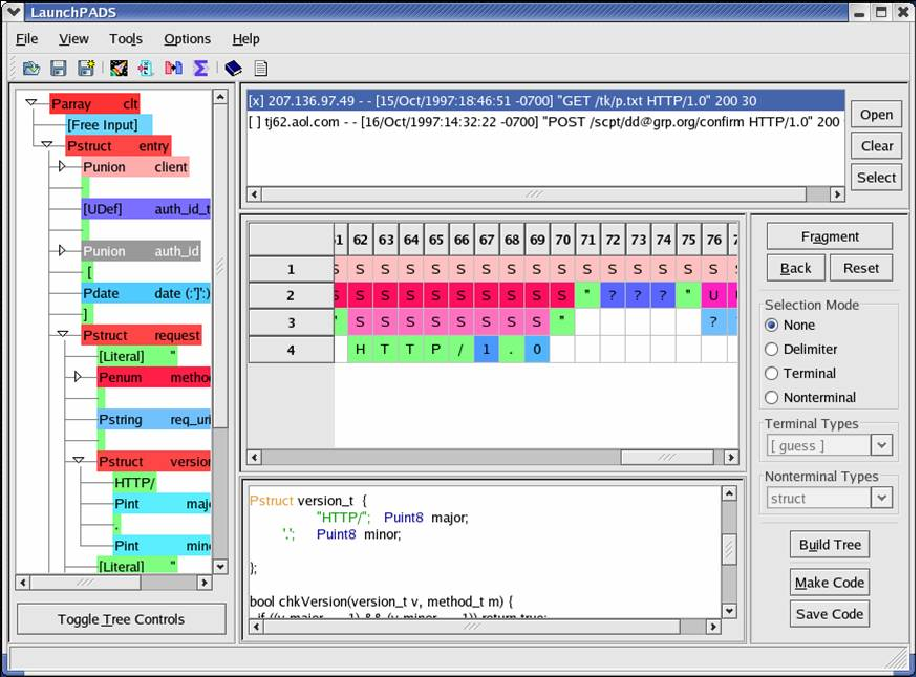
\includegraphics{launch.pdf}}
  \end{center}
  \caption{\launchpads{} Interactive User Interface.}
  \label{figure:launchpads}
\end{figure*}

When the analyst is satisfied with the description in the treeview,
she can test her description on a larger fragment of sample data.  To
do this, \launchpads{} generates syntactically correct \pads{} code,
which is shown in bottom-most frame of Figure~\ref{figure:launchpads},
and invokes the \pads{} compiler to produce a parsing library from the
generated description.  Description-independent tools are linked with
the description-dependent library and made available to the analyst
through menus in the \launchpads{} interface.  

The analyst can test her description by applying the accummulator tool
to a larger sample of data.  For each type in a \pads{} description,
accumulators report the number of good values, the number of bad
values, and the distribution of legal values.  In the \launchpads{}
interface, records identified by the accumulator as containing errors
are displayed in the data view.  The analyst can then determine
whether the errors are due to genuine errors in the data or due to
incomplete or out-of-date documentation, in which case she can refine
the description to improve its coverage.

This phase helps the analyst learn the layout and the meaning of the
data, determine the completeness of the format's documentation,
identify different representations for ``data not available'', and
learn the distribution of values for particular fields, \etc{}  When
finished with this phase, the analyst may be ready to ask some basic
queries such as ``Select all orders starting within a certain time
window,'' ``Count the number of orders going through a particular
state,'' and ``What is the average time required to go from a
particular event state to another particular event state''.  Such
queries are useful for rapid information discovery and for vetting
errors and anomalies in data before the data proceeds to a
down-stream process or is loaded into a database.

With \pads{}, the analyst uses XQuery to query her ad hoc data source.
Because XQuery is designed for semi-structured data, its
expressiveness matches ad hoc data sources well.  For example, the
analyst can write the expression below to produce all orders
that started in October, 2004.
\begin{code}
$pads/Psource/orders/elt[events/elt[1]
  [tstamp/rep {>=} {xs:date}("2004-10-01")
{and} tstamp/rep {<} {xs:date}("2004-11-01")]]
\end{code}

Existing \pads{} tools may not be solve all the analysts problems,
in which case, she may write her own \pads{} applications that call  directly
the \pads{}-generated parsing or tool libraries.  Most
importantly, her effort has produced a reusable description that she
can share with other analysts.  The fact that useful software
artifacts are generated from the descriptions provides strong
incentive for keeping the descriptions current, allowing the descriptions to serve
as living documentation.

% \Galax{}~\cite{galaxmanual}

